\documentclass[12pt, twoside]{article}
\usepackage[francais]{babel}
\usepackage[T1]{fontenc}
\usepackage[latin1]{inputenc}
\usepackage[left=7mm, right=7mm, top=7mm, bottom=7mm]{geometry}
\usepackage{float}
\usepackage{graphicx}
\usepackage{array}
\usepackage{multirow}
\usepackage{amsmath,amssymb,mathrsfs} 
\usepackage{soul}
\usepackage{textcomp}
\usepackage{eurosym}
\usepackage{lscape}
 \usepackage{variations}
\usepackage{tabvar}
 
\pagestyle{empty}

\title{\ul{\textbf{Organisation et repr�sentation des donn�es}}}
\date{}

\begin{document}
\maketitle


\section{Tableaux}

\fbox{
\begin{minipage}{18cm}
Un tableau permet de regrouper et d'organiser des donn�es, de lire facilement
des informations.
\end{minipage}
}





\subsection{Tableaux � deux lignes}


\ul{Exemple}: Les r�sultats du premier tour d'une �lection des d�l�gu�s de
classe sont not�s dans le tableau ci-dessous.

\enskip

La premi�re ligne nous donne le noms des candidats.
La deuxi�me ligne nous donne le nombre de votes obtenus.

\enskip

\begin{tabular}{cc}
\begin{minipage}{9cm}


\begin{enumerate}
  \item Qui a obtenu 5 voix? 
  
  \ldots \ldots \ldots \ldots \ldots \ldots \ldots \ldots \ldots \ldots \ldots
  \ldots \ldots \ldots 
  
  \item Qui a obtenu plus de 5 voix?
  
  \ldots \ldots \ldots \ldots \ldots \ldots \ldots \ldots \ldots \ldots \ldots
  \ldots \ldots \ldots  
  
  \item Combien Louis a-t-il  obtenu de voix?
  
  \ldots \ldots \ldots \ldots \ldots \ldots \ldots \ldots \ldots \ldots \ldots
  \ldots \ldots \ldots  
  \item Combien y a t-il d'�l�ves dans cette classe?
  
  \ldots \ldots \ldots \ldots \ldots \ldots \ldots \ldots \ldots \ldots \ldots
  \ldots \ldots \ldots  

\end{enumerate}
\end{minipage}
&
\begin{minipage}{9cm}
\begin{center}
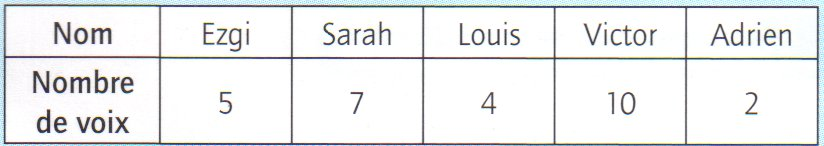
\includegraphics[width=8cm]{images/ligne.jpg}
\end{center}
\end{minipage}
\end{tabular}

\subsection{Tableaux � deux colonnes}

\ul{Exemple}: Voici un extrait du tarif postal pour affranchir des lettres.

\enskip

La premi�re colonne nous donne les diff�rentes cat�gories de poids.
La deuxi�me colonne nous indique le tarif.

\enskip


\begin{tabular}{cc}
\begin{minipage}{14cm}

\begin{enumerate}
  \item Combien co�te l'envoi d'une lettre de 15g? 
  
  \ldots \ldots \ldots \ldots \ldots \ldots \ldots \ldots
  \ldots \ldots \ldots \ldots  \ldots \ldots \ldots \ldots \ldots \ldots
  \item Combien co�te l'envoi d'une lettre qui p�se deux fois plus?
  
    \ldots \ldots \ldots \ldots \ldots \ldots \ldots \ldots
  \ldots \ldots \ldots \ldots  \ldots \ldots \ldots \ldots \ldots \ldots  
  
  \item Pour quel masse paye-t-on 1,33 \euro?

  \ldots \ldots \ldots \ldots \ldots \ldots \ldots \ldots
  \ldots \ldots \ldots \ldots  \ldots \ldots \ldots \ldots \ldots \ldots
\end{enumerate}
\end{minipage}
&
\begin{minipage}{4cm}
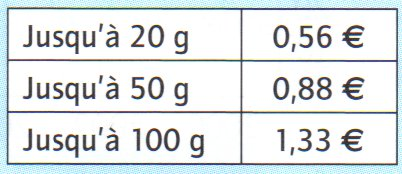
\includegraphics[width=4cm]{images/colonne.jpg}
\end{minipage}
\end{tabular}

\subsection{Tableaux � double entr�e}

\ul{Exemple}:

\begin{tabular}{cc}
\begin{minipage}{12cm}
\begin{enumerate}
  \item La ligne gris�e donne le nombre d'�l�ves qui ont  \ldots \ldots dans
  les classes de $6^{e}$.
  \item La colonne gris�e donne la r�partition des �l�ves de $6^{e}\ldots$
  selon leur �ge.
  \item Combien d'�l�ves de $6^{e}2$ ont 12 ans?
  
  \ldots \ldots \ldots \ldots \ldots \ldots \ldots \ldots \ldots \ldots \ldots
  \ldots \ldots \ldots \ldots \ldots \ldots \ldots \ldots \ldots
  
  \item Parmi les �l�ves qui ont 13 ans, quels sont ceux qui sont en $6^{e}1$?
  
  \ldots \ldots \ldots \ldots \ldots \ldots \ldots \ldots \ldots \ldots \ldots
  \ldots \ldots \ldots \ldots \ldots \ldots \ldots \ldots \ldots
\end{enumerate}
\end{minipage}
&
\begin{minipage}{6cm}
\begin{center}
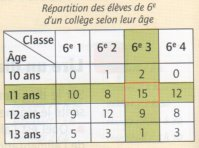
\includegraphics[width=5cm]{images/double.jpg}
\end{center}
\end{minipage}
\end{tabular}
\section{Graphique cart�sien}


\fbox{
\begin{minipage}{18cm}
Un graphique cart�sien permet de visualiser l'\textbf{�volution} d'une grandeur
en fonction d'une autre.
\end{minipage}
}


\enskip

\ul{Exemple}:


\begin{center}
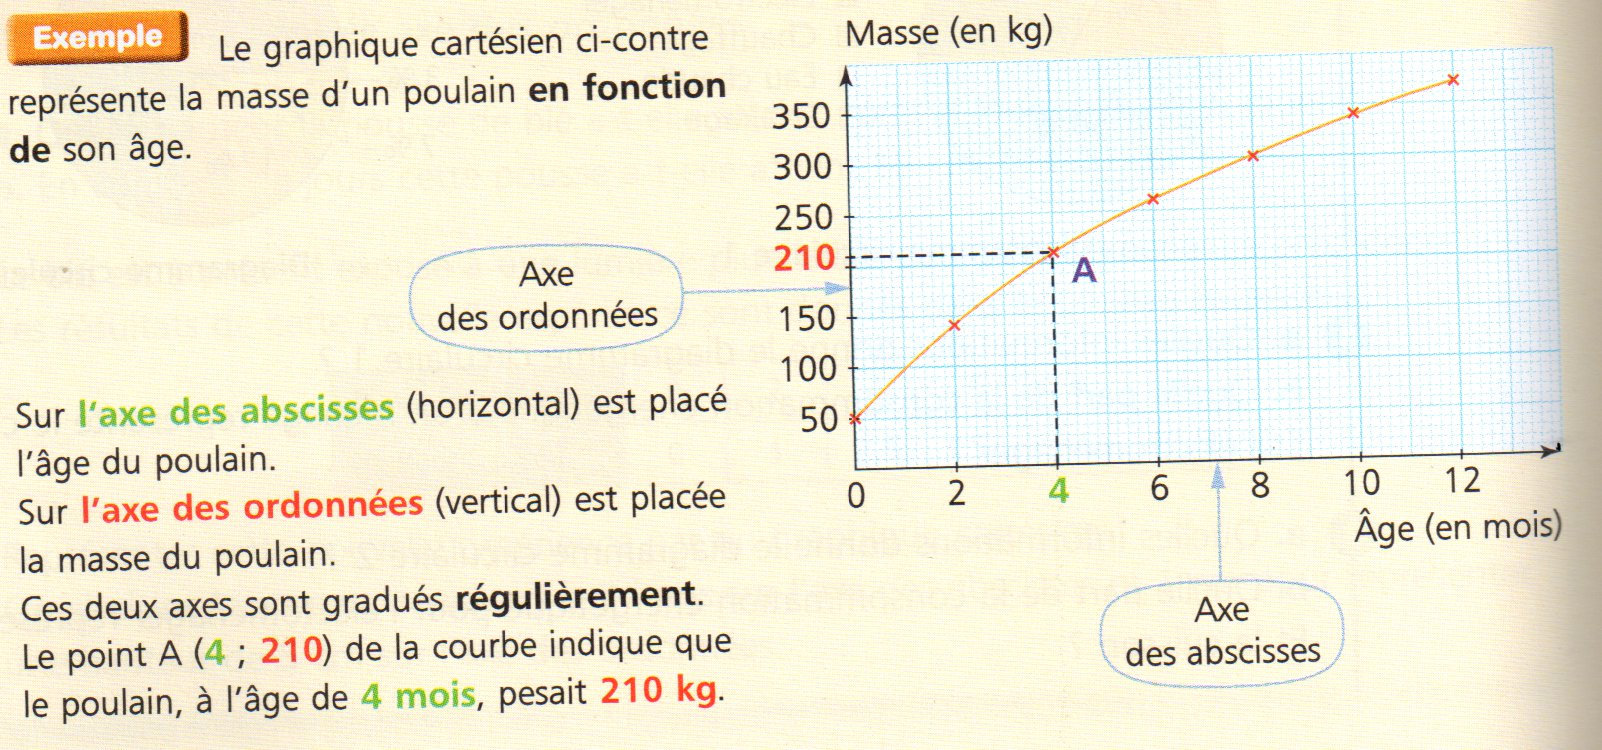
\includegraphics[width=15cm]{images/graphique.jpg}
\end{center}


\enskip


\begin{enumerate}
  \item Combien p�se le poulain � l'�ge de 8 mois?
  
  \ldots \ldots \ldots \ldots \ldots \ldots \ldots \ldots \ldots \ldots \ldots
  \ldots \ldots \ldots \ldots \ldots \ldots \ldots \ldots \ldots   \ldots
  \ldots \ldots \ldots \ldots \ldots \ldots \ldots \ldots \ldots \ldots \ldots
  \ldots \ldots \ldots 
  
  \item A partir de quel �ge, le poulain p�se-til plus de 100 kg?
  
  \ldots \ldots \ldots \ldots \ldots \ldots \ldots \ldots \ldots \ldots \ldots
  \ldots \ldots \ldots \ldots \ldots \ldots \ldots \ldots \ldots   \ldots
  \ldots \ldots \ldots \ldots \ldots \ldots \ldots \ldots \ldots \ldots \ldots
  \ldots \ldots \ldots 
\end{enumerate}
\end{document}
